\title{Note on estimating the error of the extracted time resolution of the FTOF12 panel 1b using the automated 6-bar analysis program
error analysis of the extracted time resolution using the automated 6-bar analysis program}
\date{July 05, 2015}

\documentclass[12pt]{article}

\usepackage{hyperref}
\usepackage{cite}

\usepackage{graphicx}
\usepackage{epsfig}
\usepackage{epstopdf}

\usepackage[pdf]{pstricks}

\usepackage{mathtools}
\newcommand{\defeq}{\vcentcolon=}

\usepackage{float}
\restylefloat{table}

%! To create a place-holder figure
\newcommand{\dummyfig}[1]{
  \centering
  \fbox{
    \begin{minipage}[c][0.33\textheight][c]{0.5\textwidth}
      \centering{#1}
    \end{minipage}
  }
}

\begin{document}
\maketitle

% \begin{abstract}
% This is the paper's abstract \ldots
% \end{abstract}

 
\section{Introduction}

Estimating the true error of the extracted time resolution of the system requires a thorough analysis of the statistical and non-statistical uncertainties. Given the scale of the project and therefore, constraints on the time it was not possible to, during production, estimate even the true statistical error of the system. In this section is described the method that was used post production using a set of reference counters -- 6x210cm bars(half slow, half fast) and 1st article PMTs -- to estimate the true statistical error for 210cm counters and then extrapolate them to bars of all lengths. This extrapolation also includes the effect of non-statistical sources of errors in the measurement, for example those pertaining to the physical properties of the counters themselves. 

Before describing the method and showing the results, the manifestation of the time constraint on the measurement and analysis procedure during production and how they affect the extraction of the true statistical errors are described in the following sub sections.

\subsection{Limited statistics in 6-bar-method measurements}
For each bar length, even after 2 days of data taking the statistics in the T histogram (\textit{refer to formula# in doc.}) are low and therefore, the statistical methods that can be used to fit and obtain the standard deviation of these histograms, which is the time resolution, has to be studied since each method, in the low statistic limit, has its own limitation in estimating the true standard deviation and its error. 

Figure 1. shows the statistics accumulated (N) for the shortest and longest counters versus points along the bar. Subsequent figures show a comparison of the various fitting methods available in ROOT for extracting $\mu$ and $\sigma$ from simulated Gaussian histograms ($\mu_{T}$ and $\sigma_{T}$) for N values between 100 and 600, reflecting the low and high end of the statistics versus bar length as can be seen in Figure 1. The $\sigma_{T}$ simulated is based on the standard deviation of the T-histogram typical for FTOF12 counters that use bar length of 210cm (\textit{confirm this!}).

\begin{figure*}[ht]
	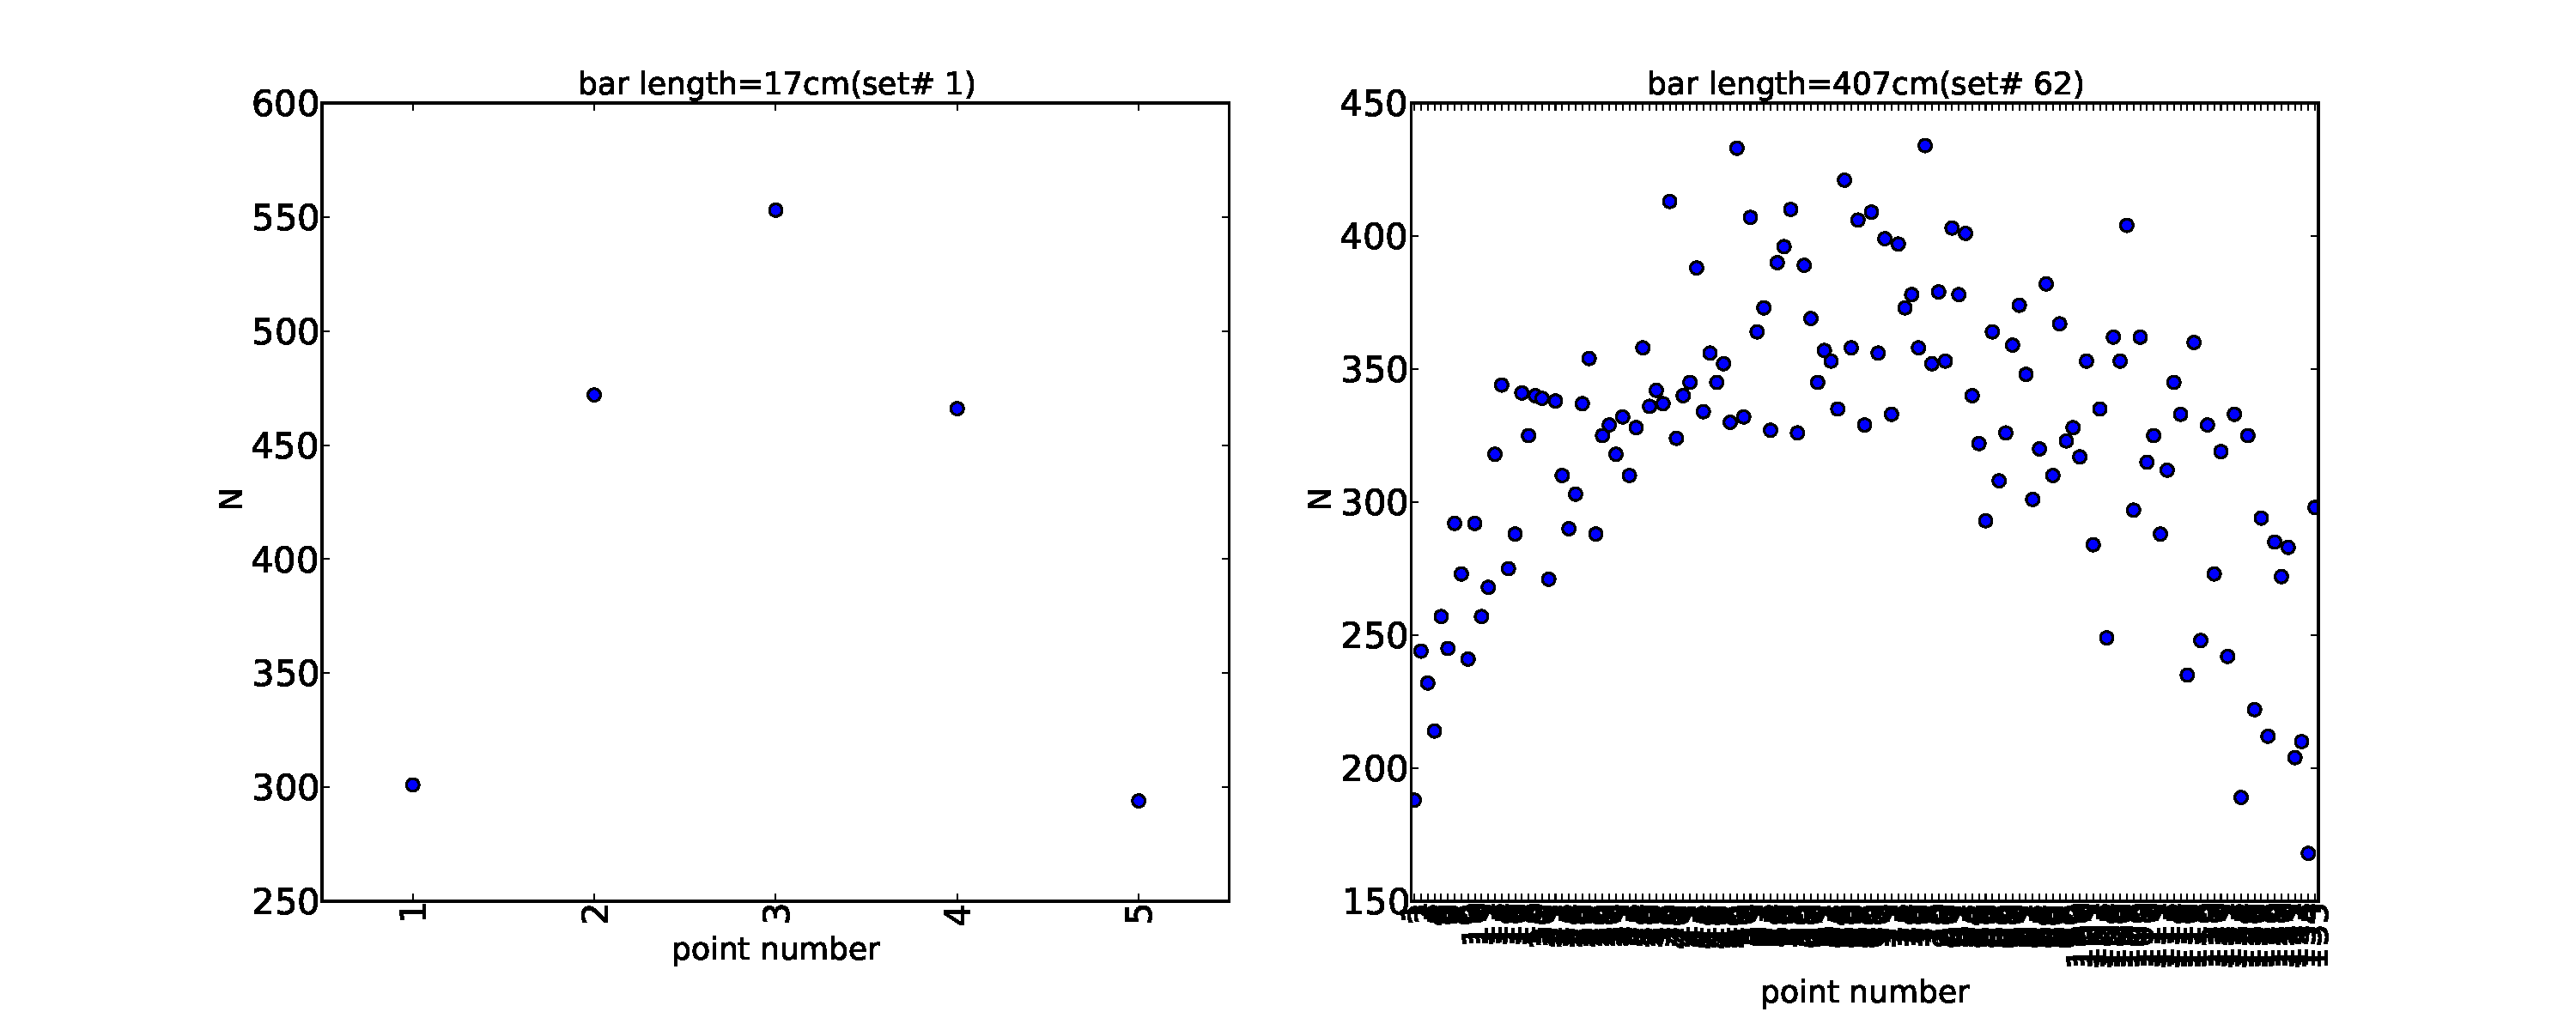
\includegraphics[height=2in,width=5in]{bar_stats_write-up_N-vs-p.pdf}
	\caption{N vs. P for the shortest and longest counters}
	\label{fig1}
\end{figure*}

\begin{figure*}[ht]
	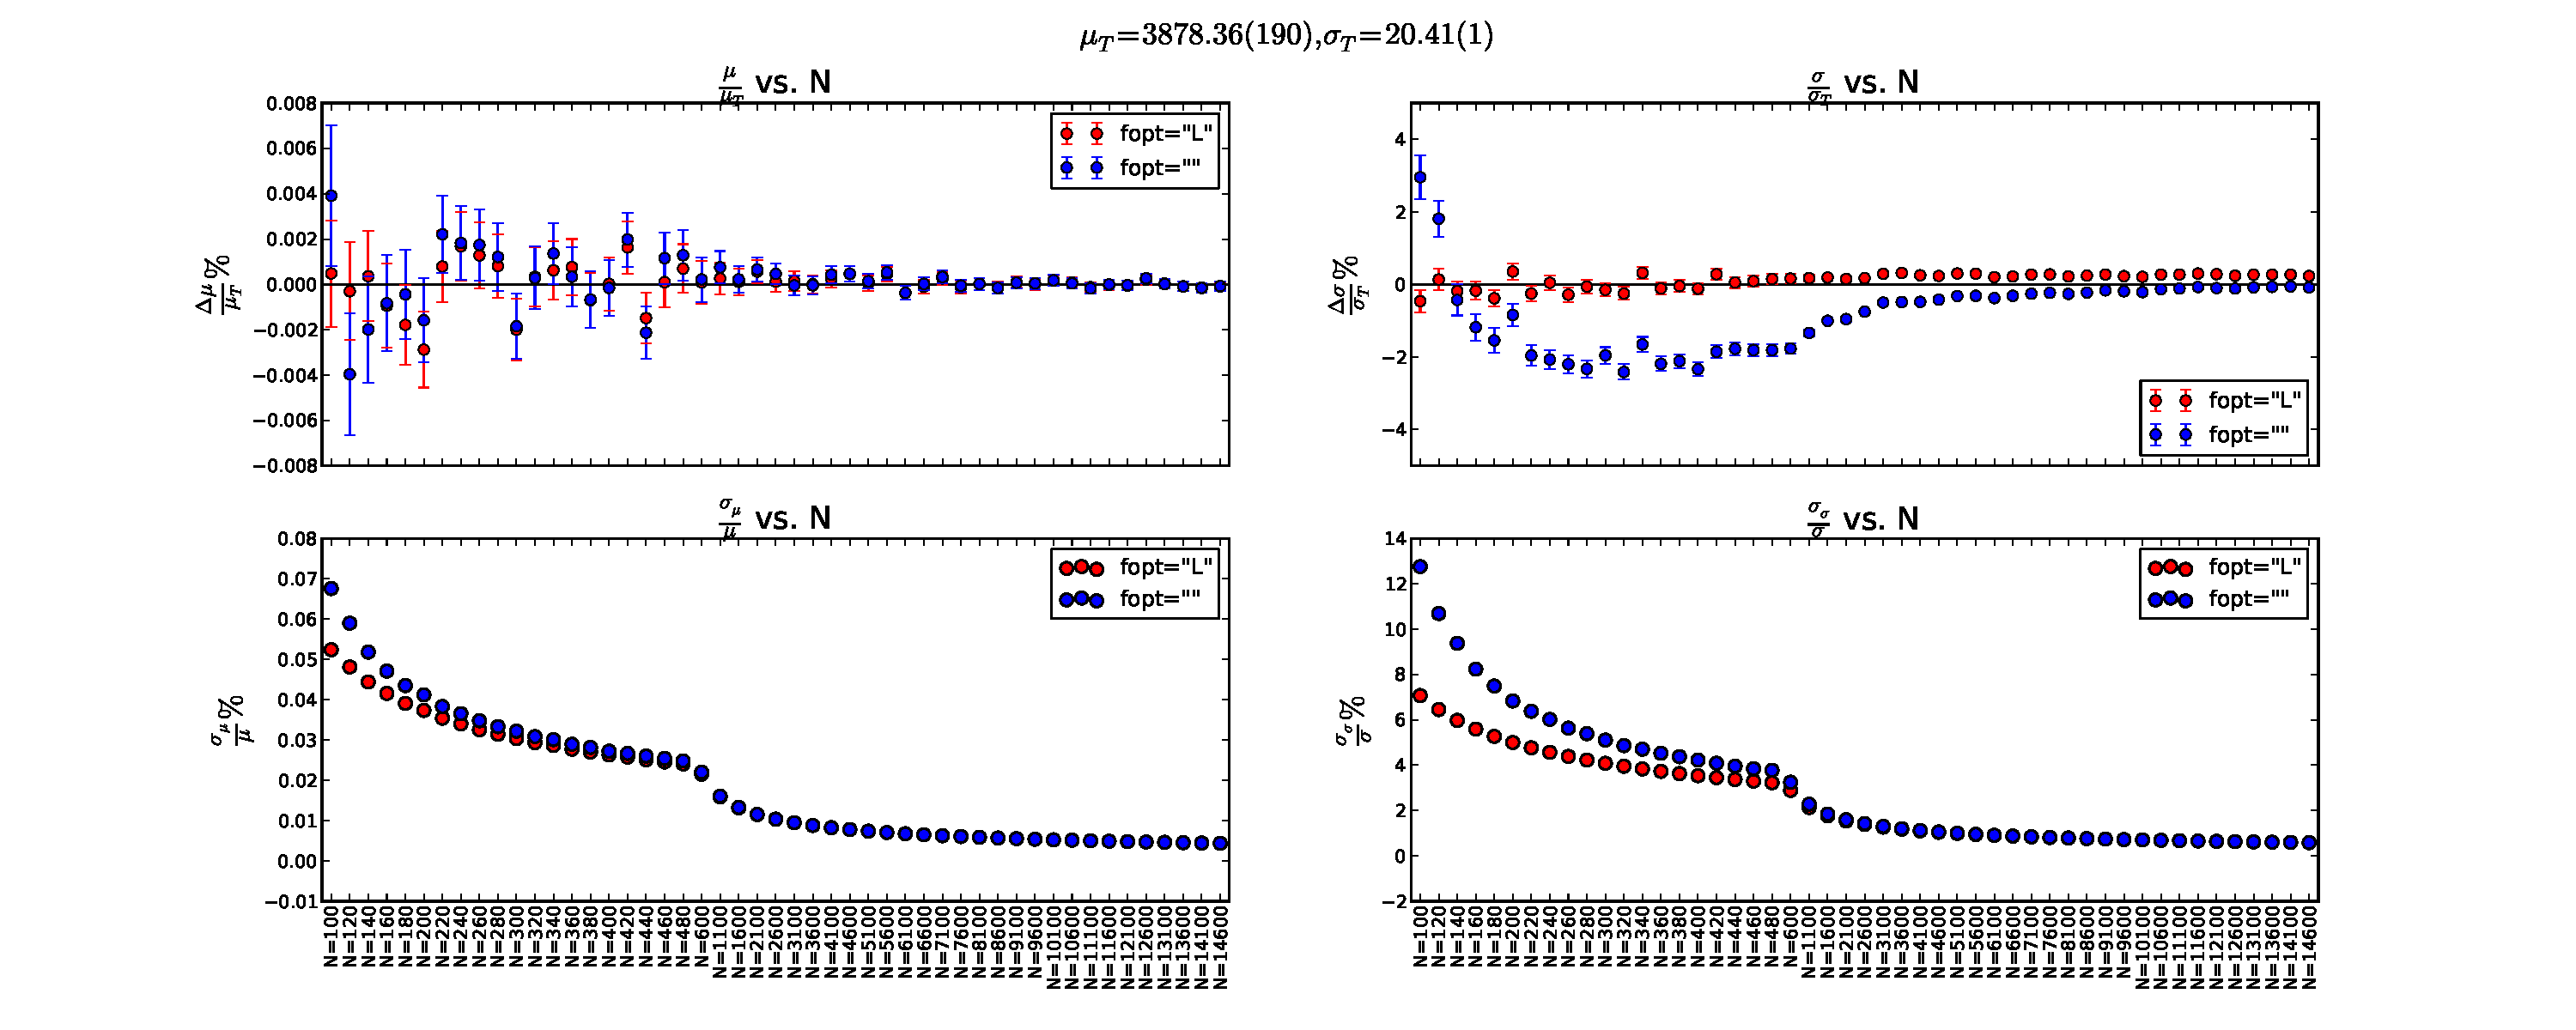
\includegraphics[height=2.5in,width=5.5in]{fit-comp_MU-190_SG-1_fit-opt-L_binw-025.pdf}
	%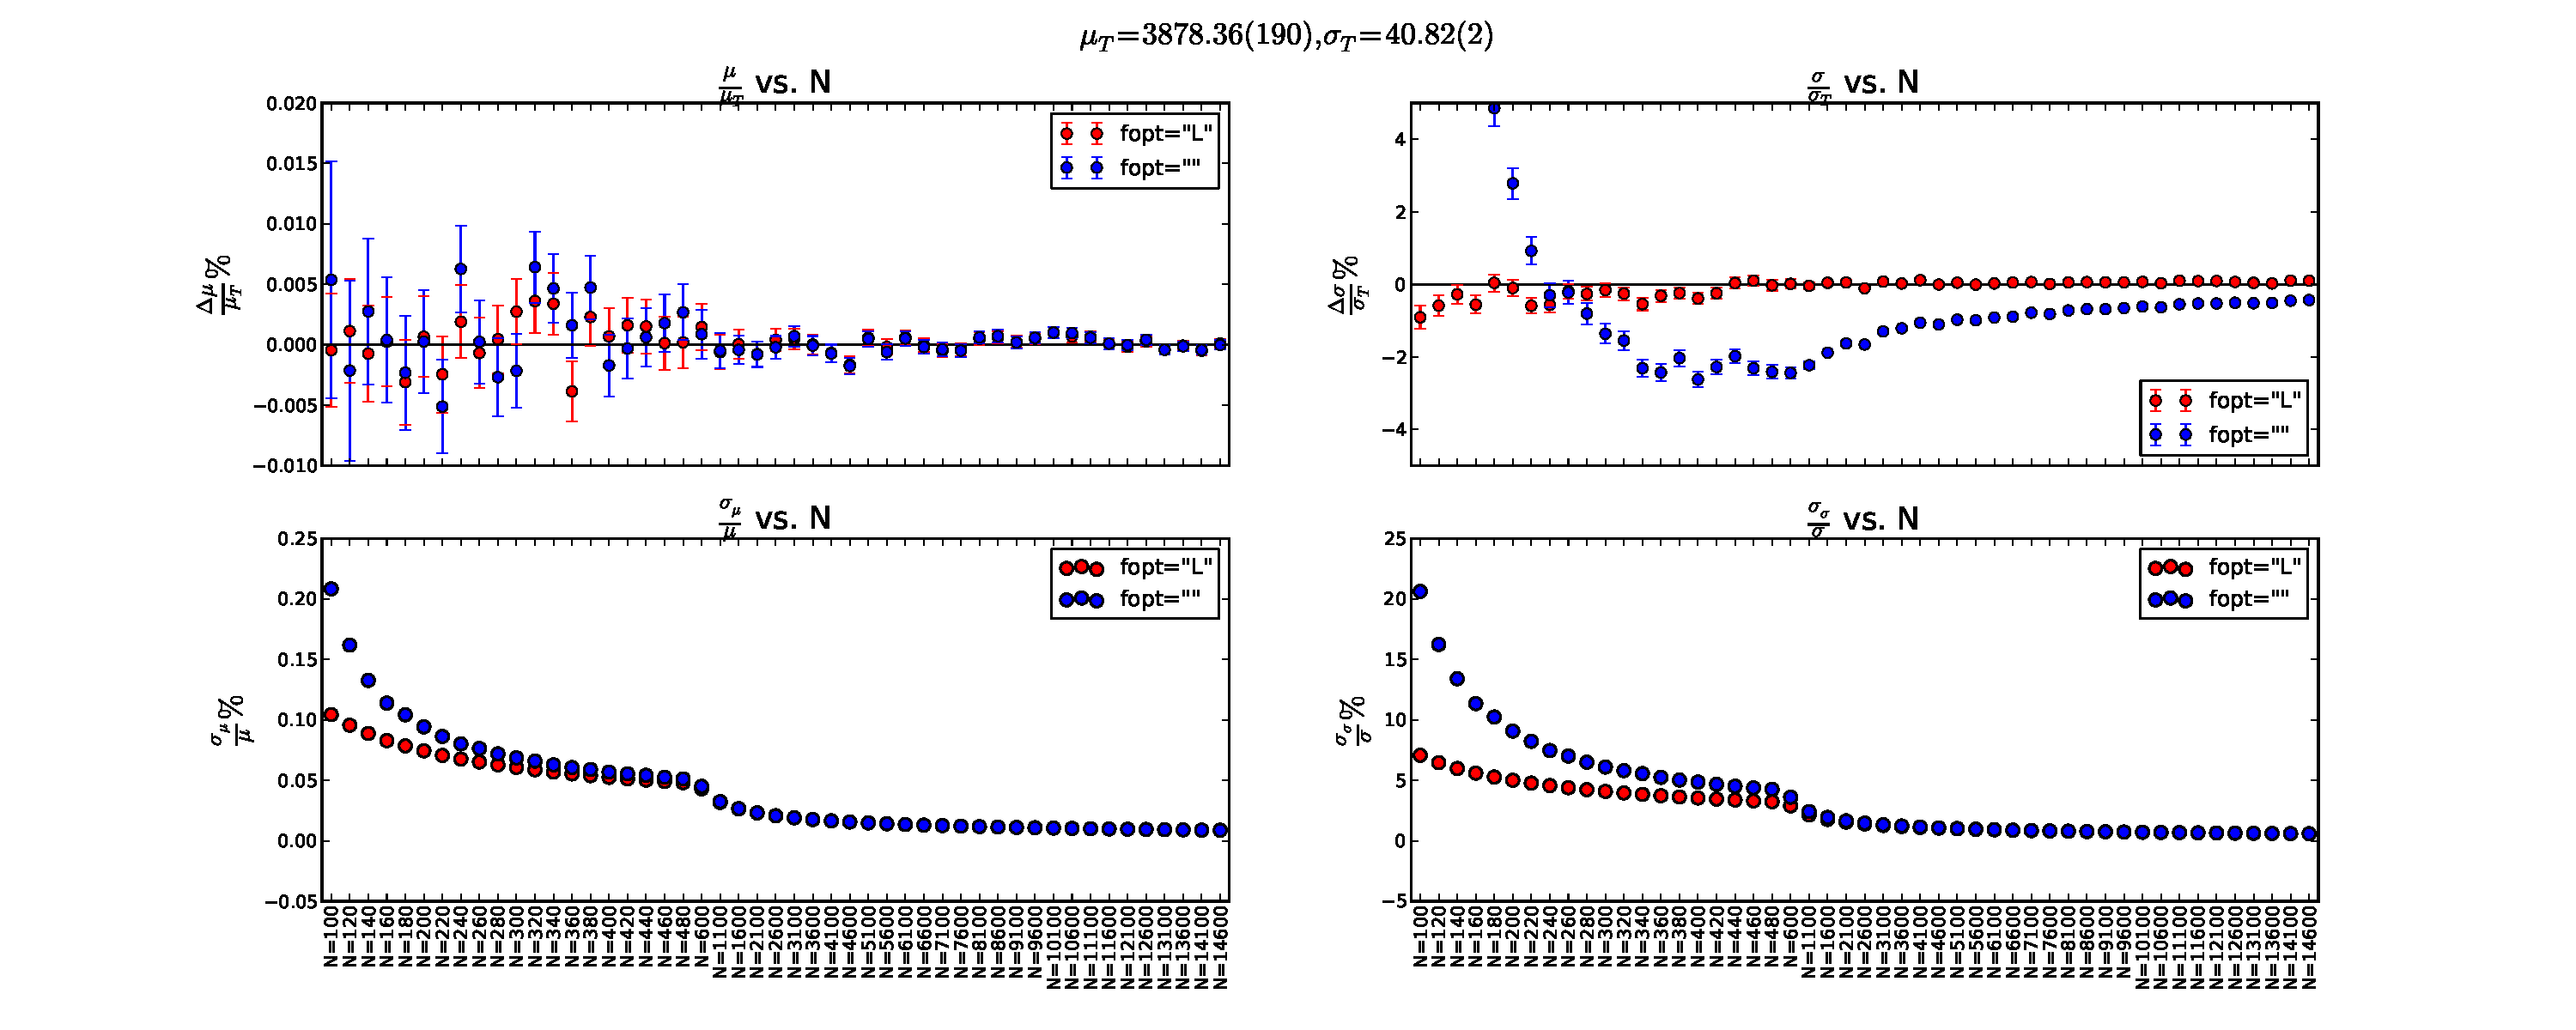
\includegraphics[height=2.5in,width=5.5in]{fit-comp_MU-190_SG-2_fit-opt-L_binw-025.pdf}
	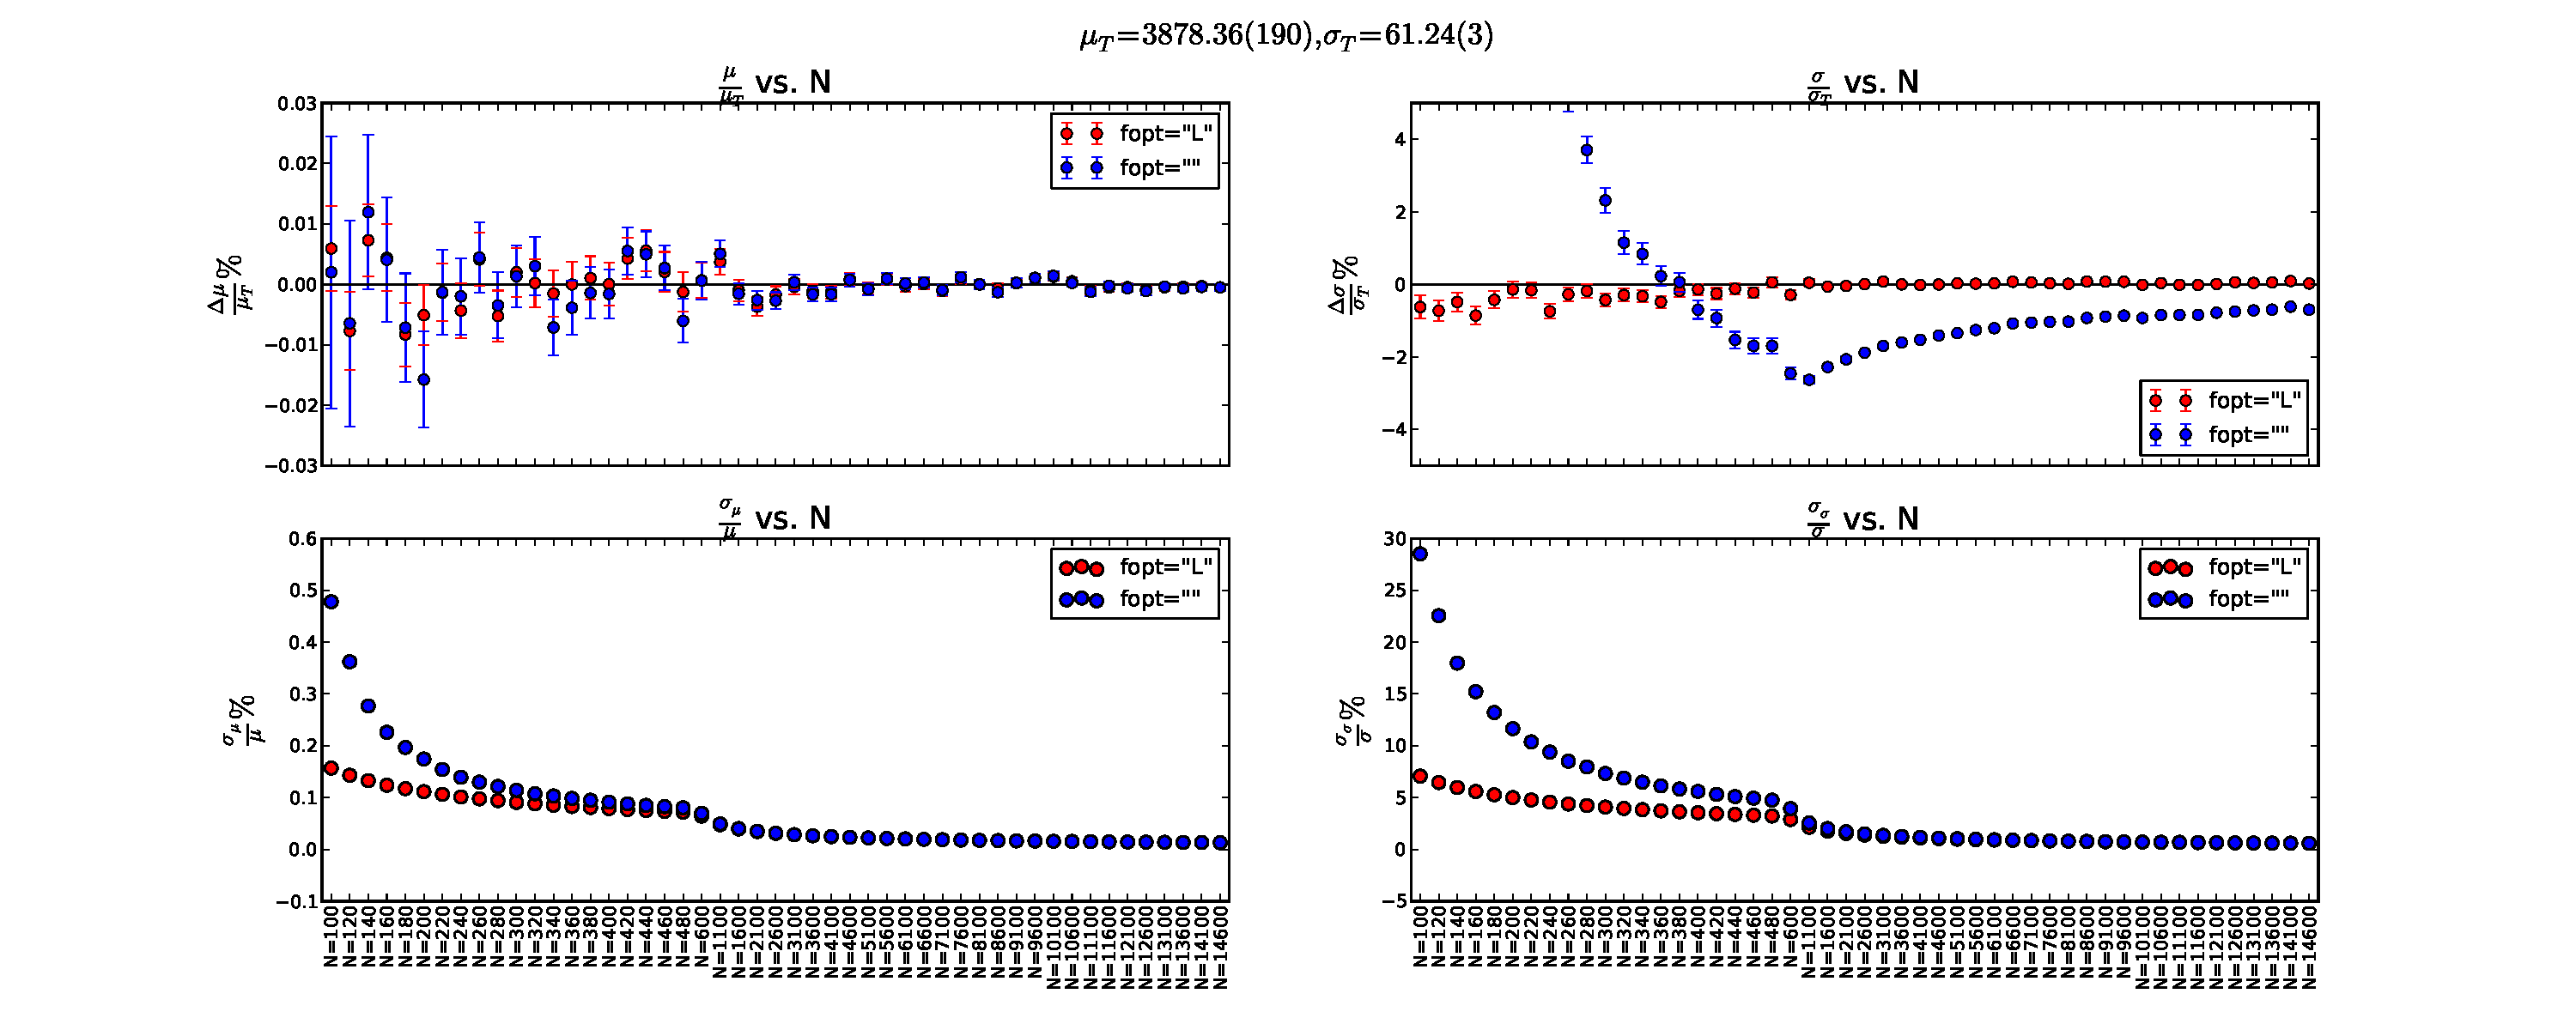
\includegraphics[height=2.5in,width=5.5in]{fit-comp_MU-190_SG-3_fit-opt-L_binw-025.pdf}
	%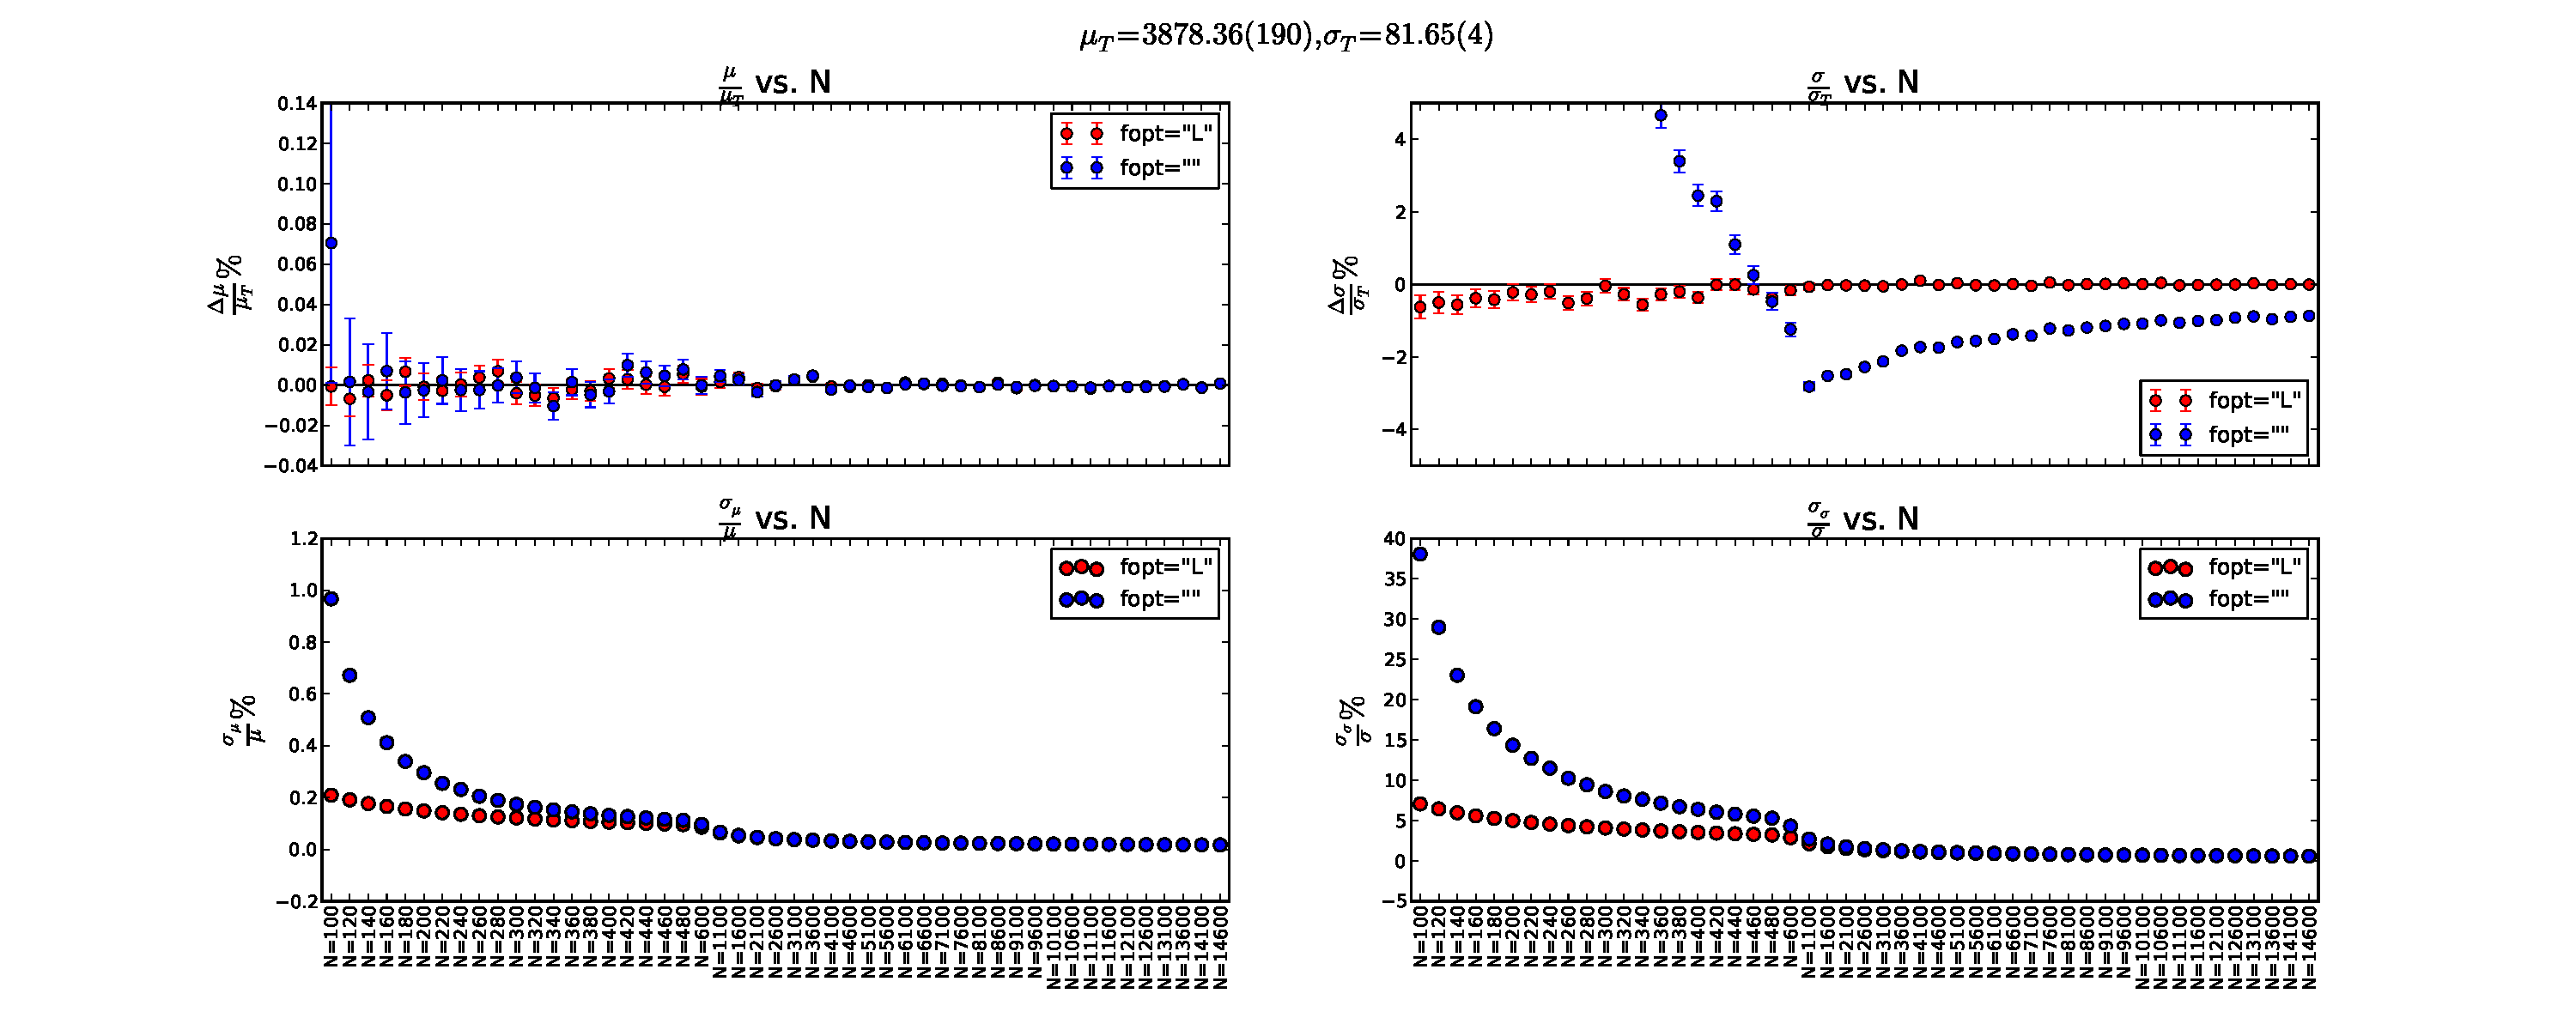
\includegraphics[height=2.5in,width=5.5in]{fit-comp_MU-190_SG-4_fit-opt-L_binw-025.pdf}
	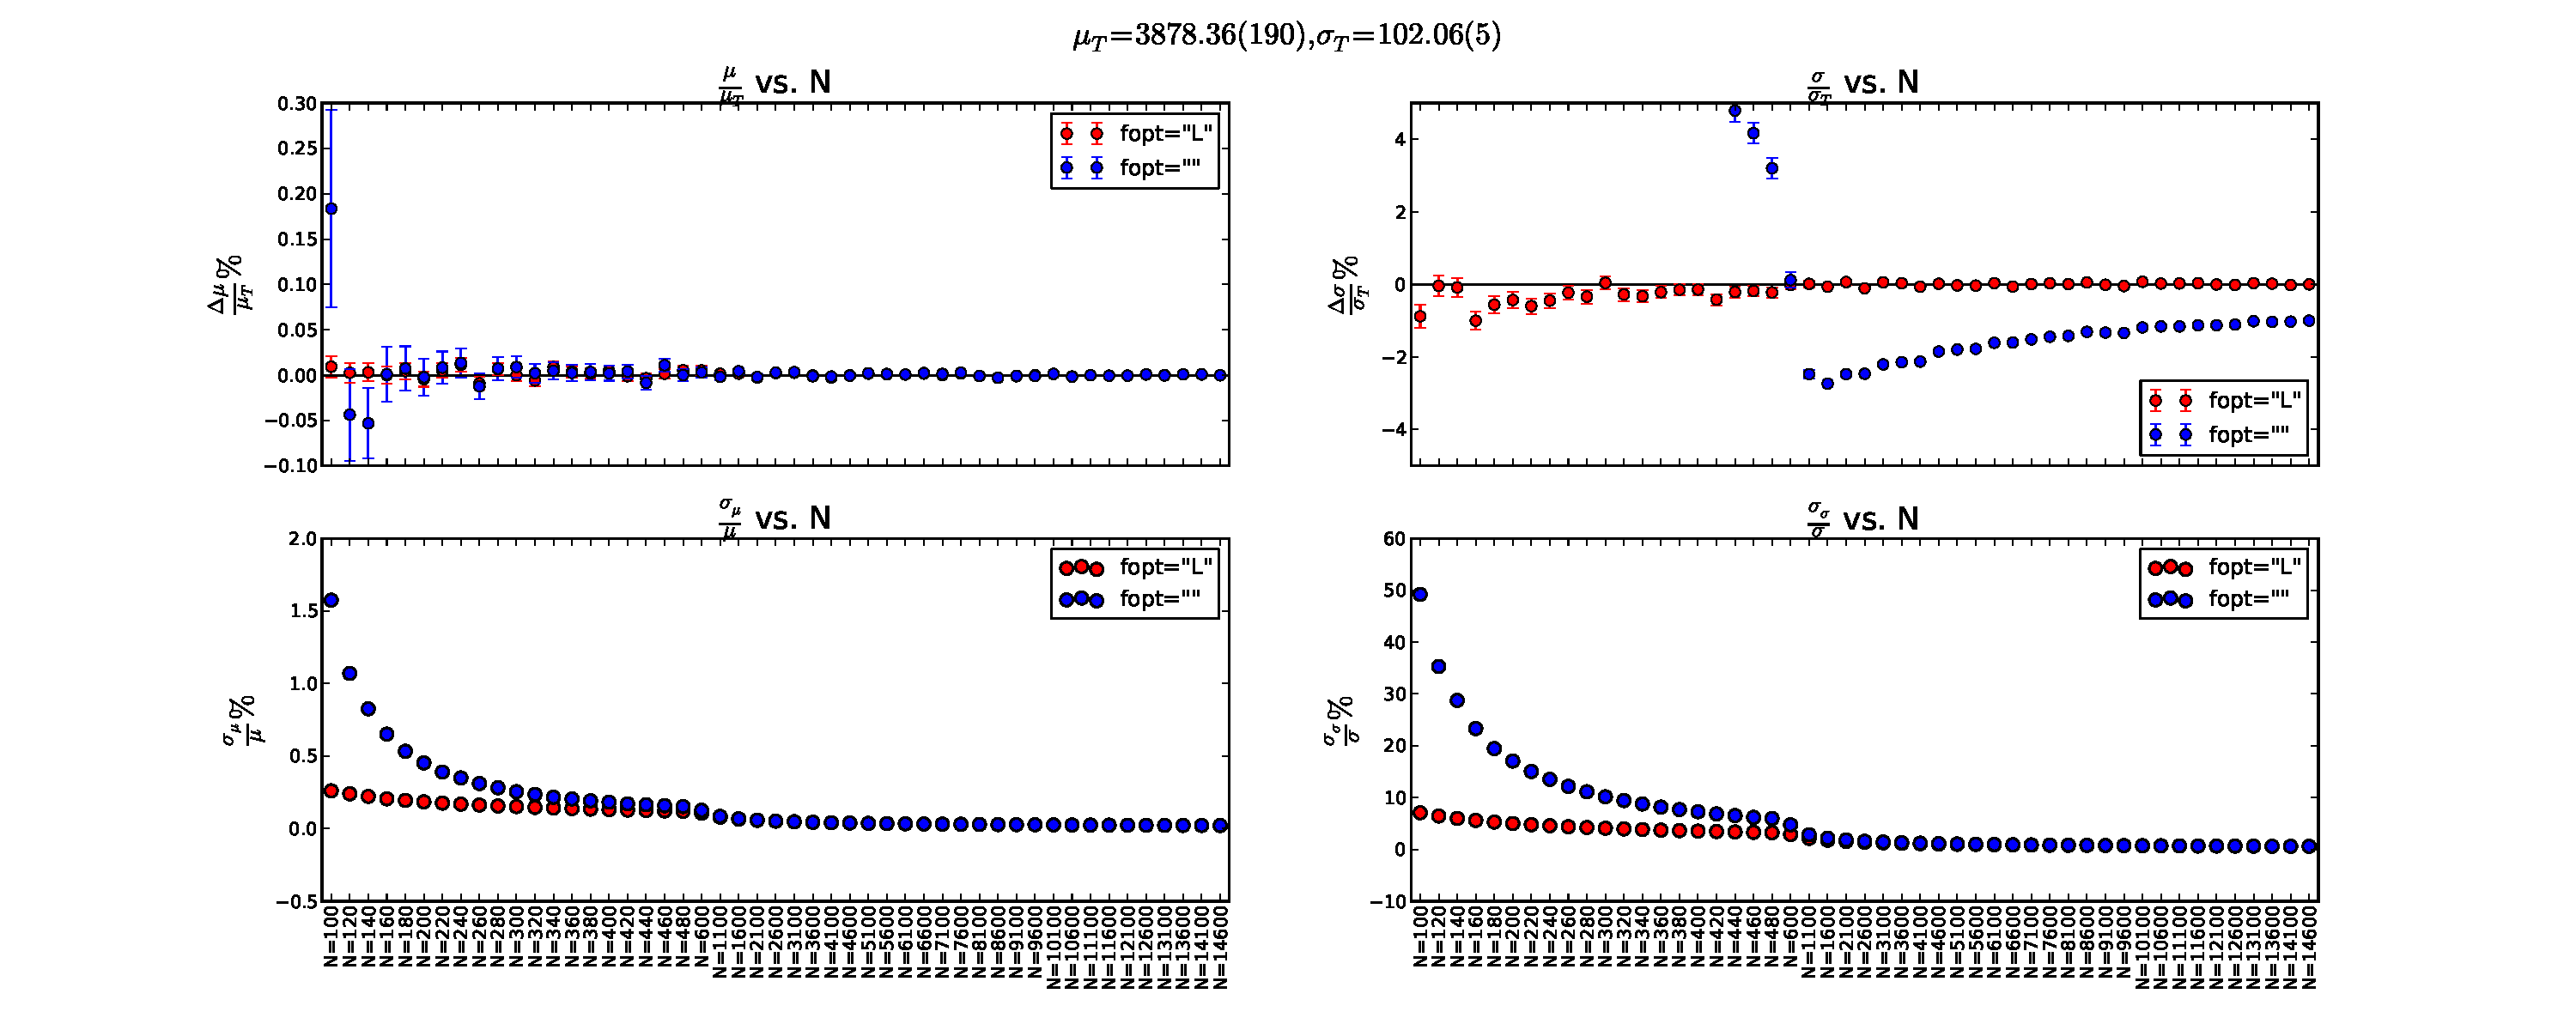
\includegraphics[height=2.5in,width=5.5in]{fit-comp_MU-190_SG-5_fit-opt-L_binw-025.pdf}
	\caption{Extracted parameters (MLE and CSQ) as a function of N and $\sigma_{T}$}
	\label{fig2}
\end{figure*}

\clearpage

\begin{figure*}[ht]
	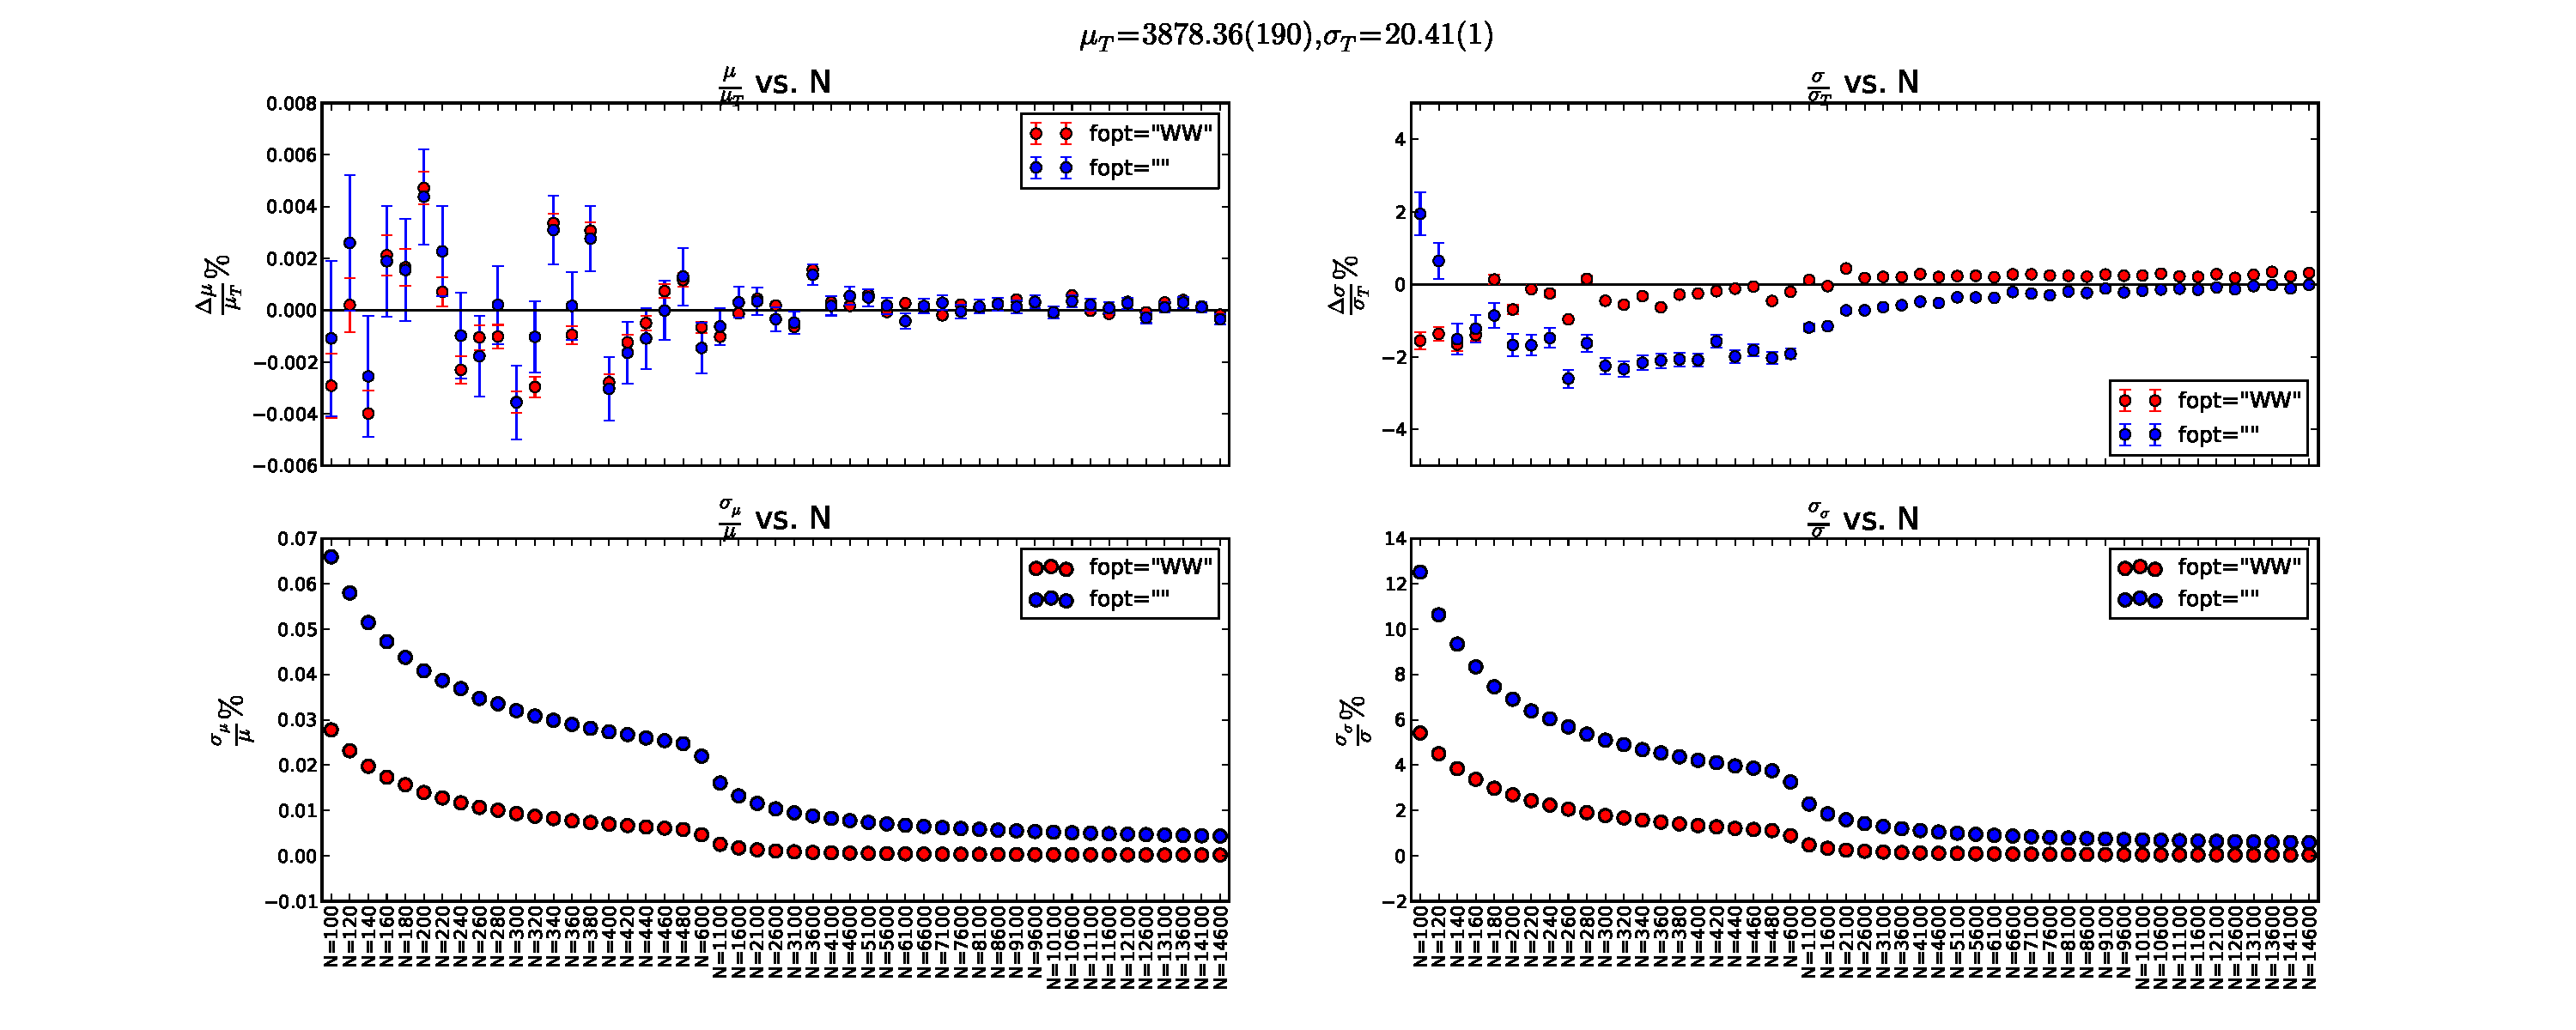
\includegraphics[height=2.5in,width=5.5in]{fit-comp_MU-190_SG-1_fit-opt-WW_binw-025.pdf}
	%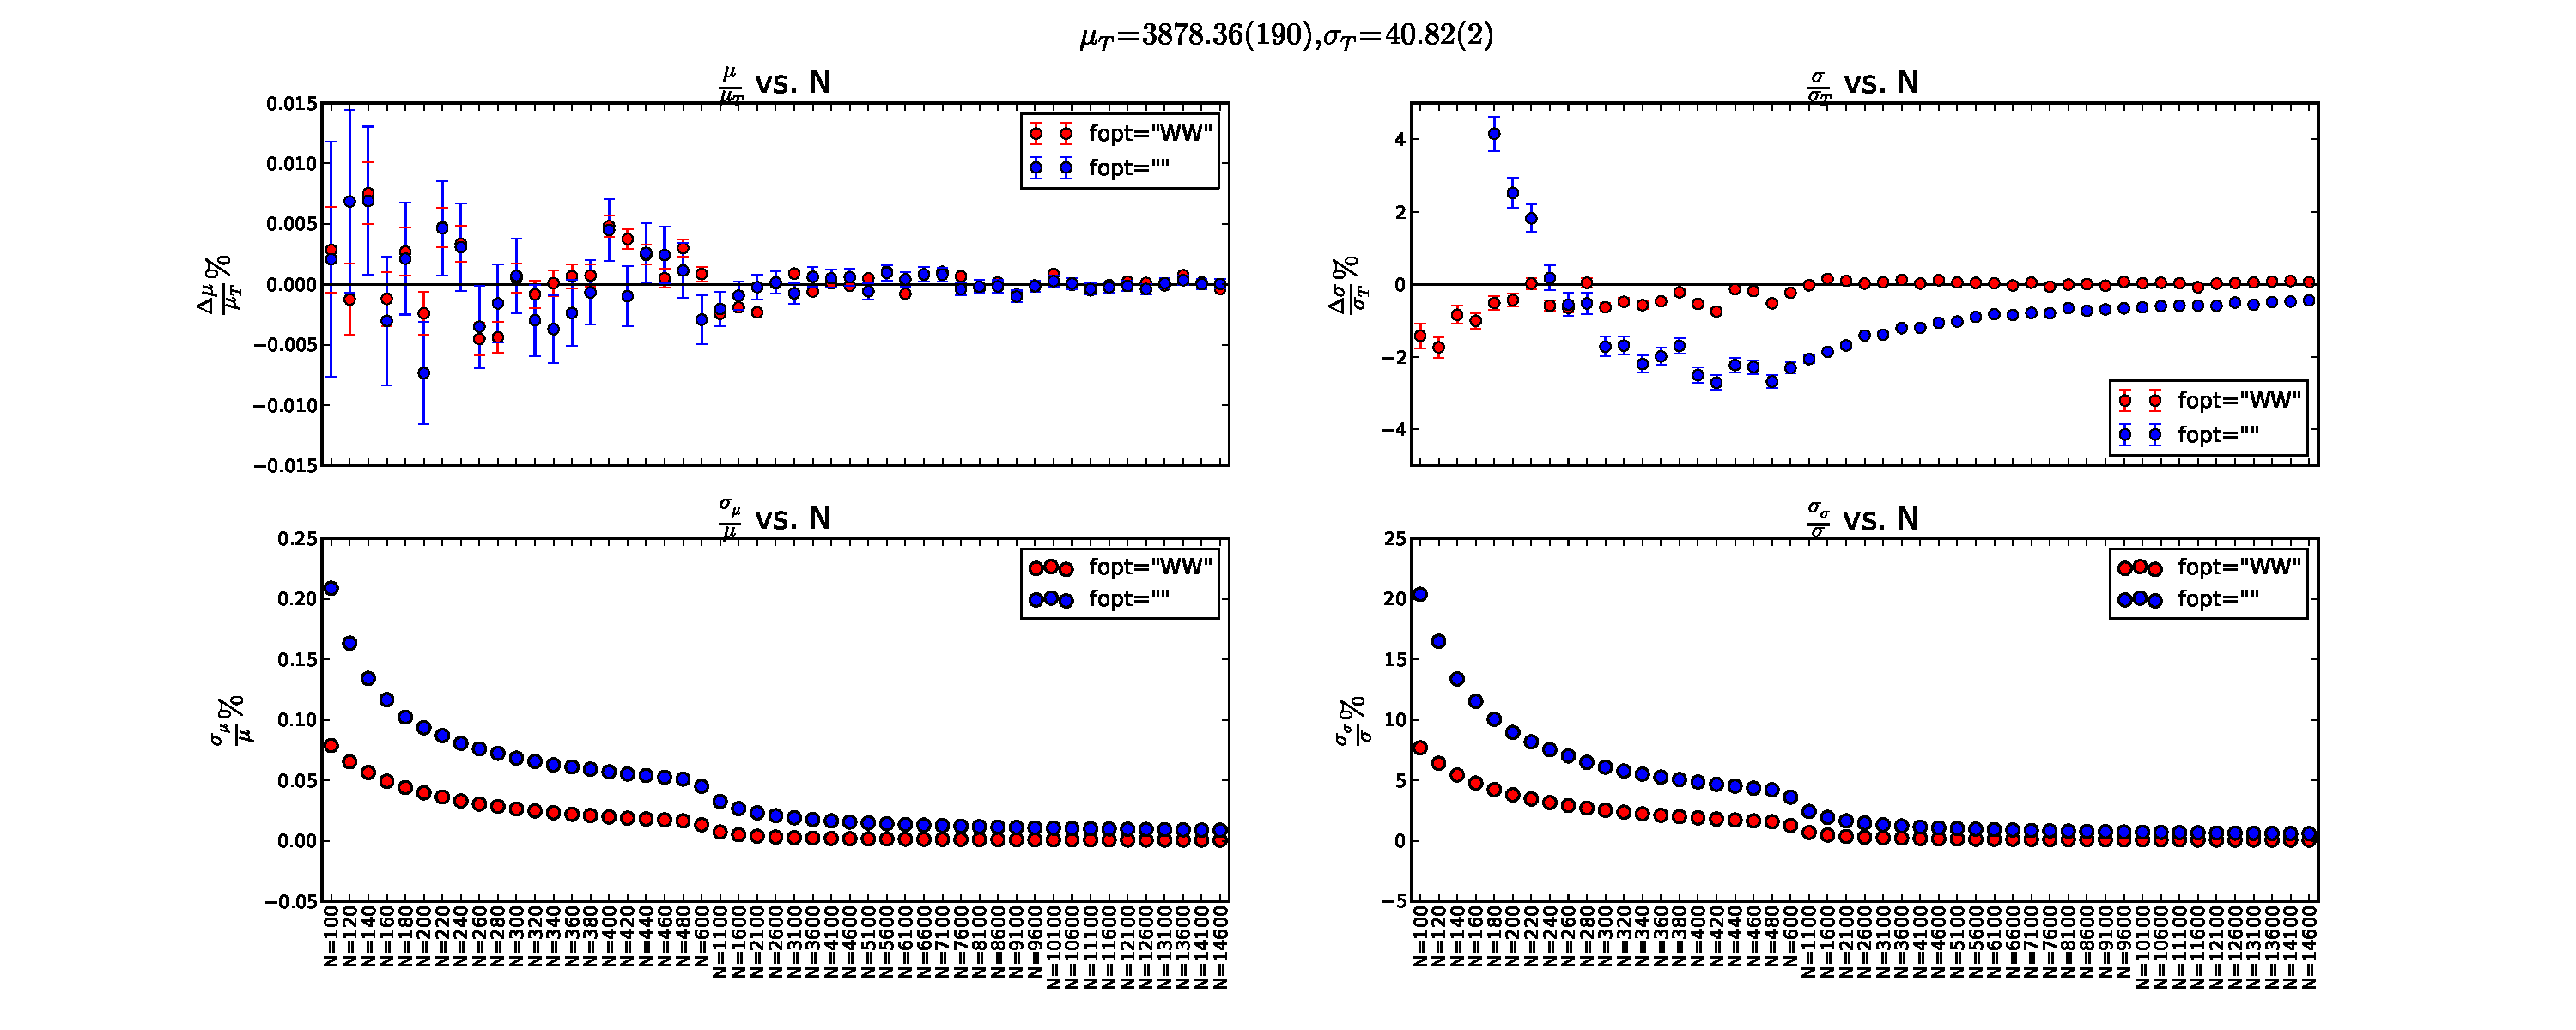
\includegraphics[height=2.5in,width=5.5in]{fit-comp_MU-190_SG-2_fit-opt-WW_binw-025.pdf}
	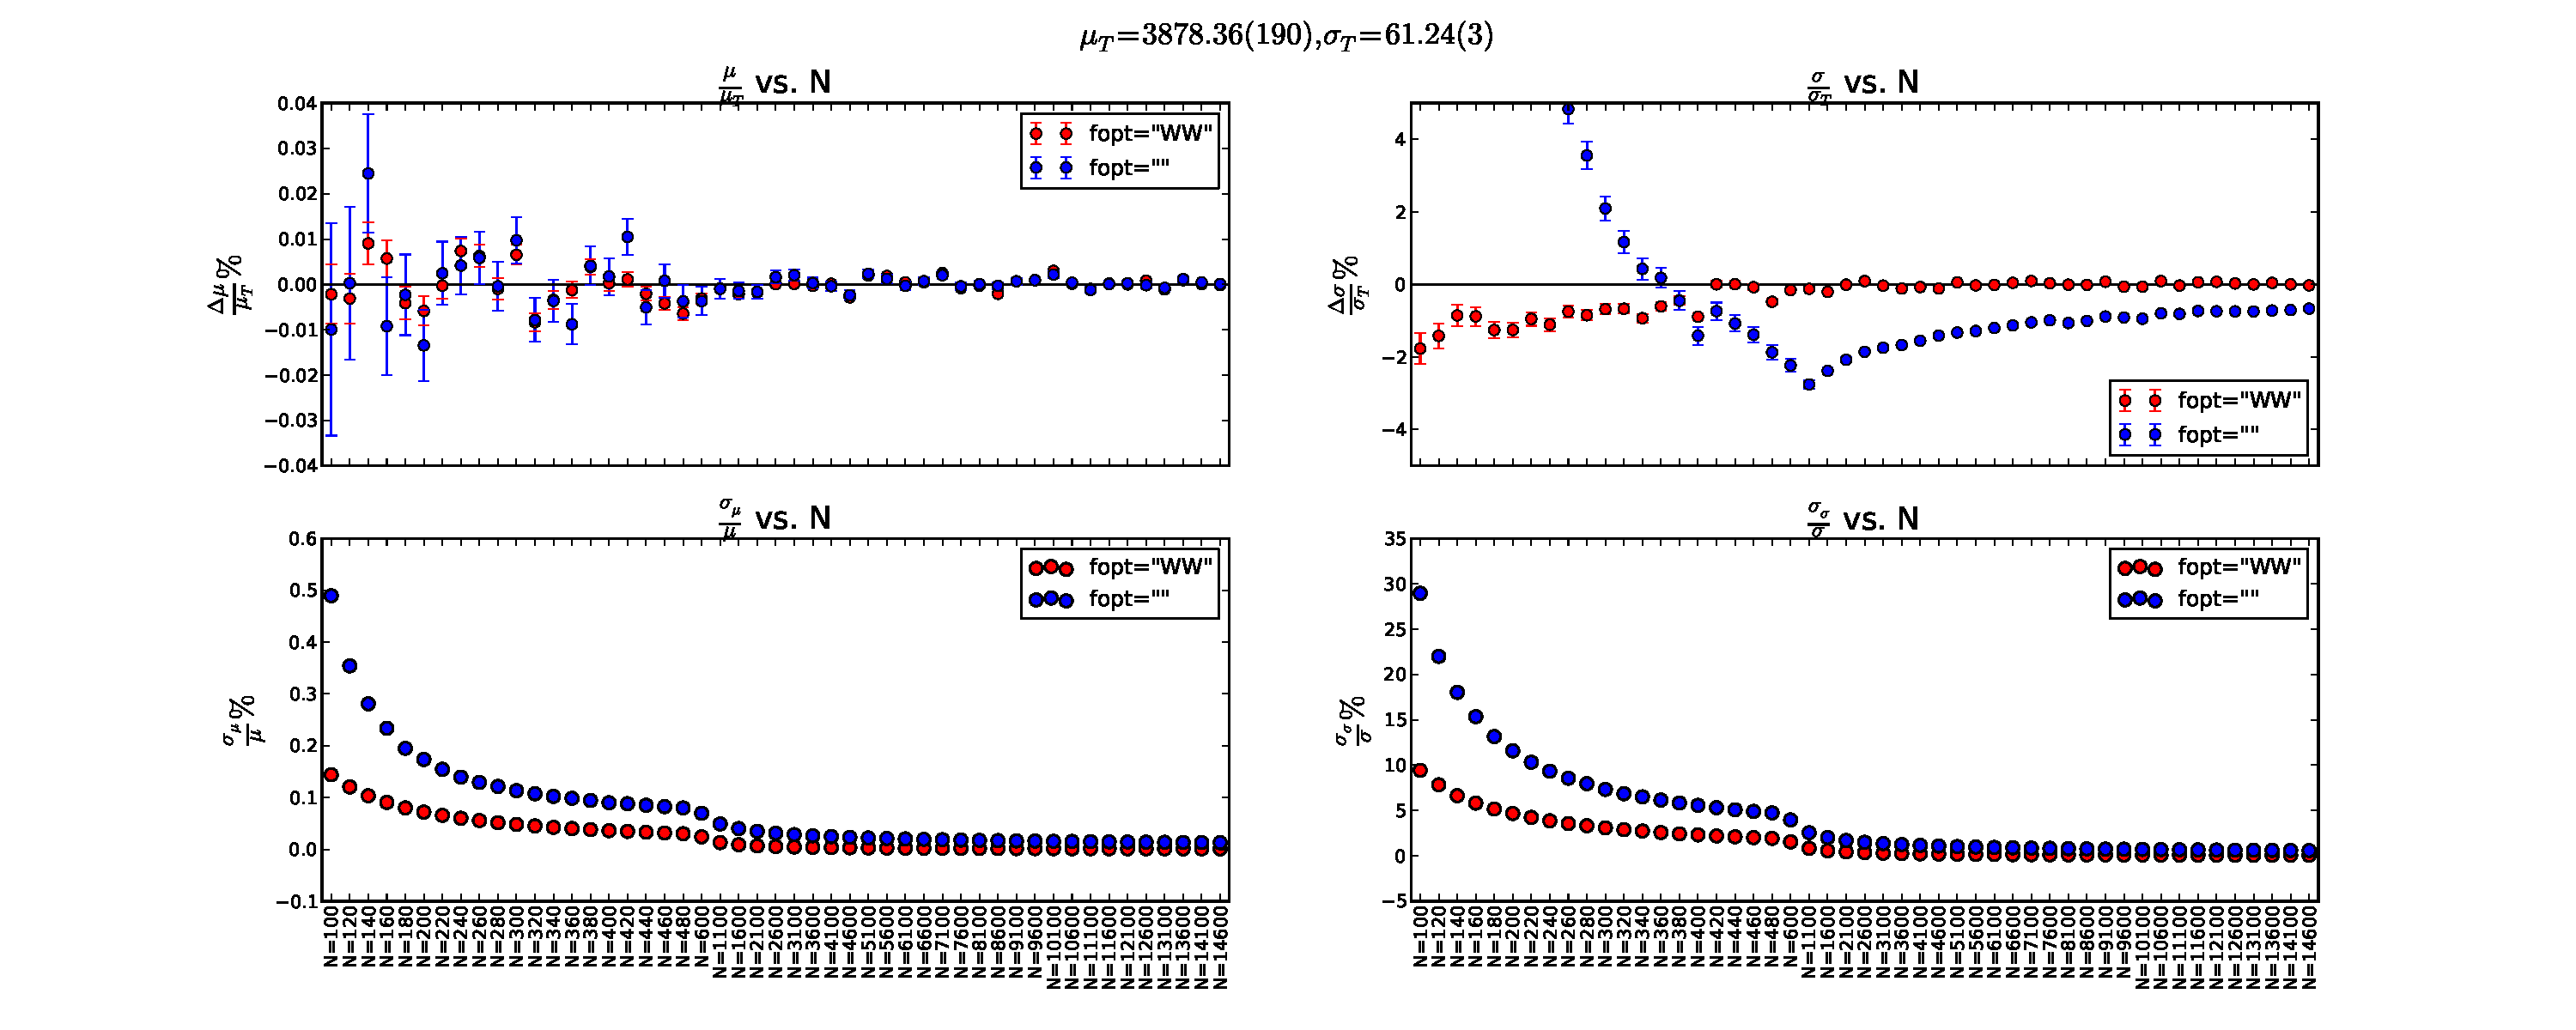
\includegraphics[height=2.5in,width=5.5in]{fit-comp_MU-190_SG-3_fit-opt-WW_binw-025.pdf}
	%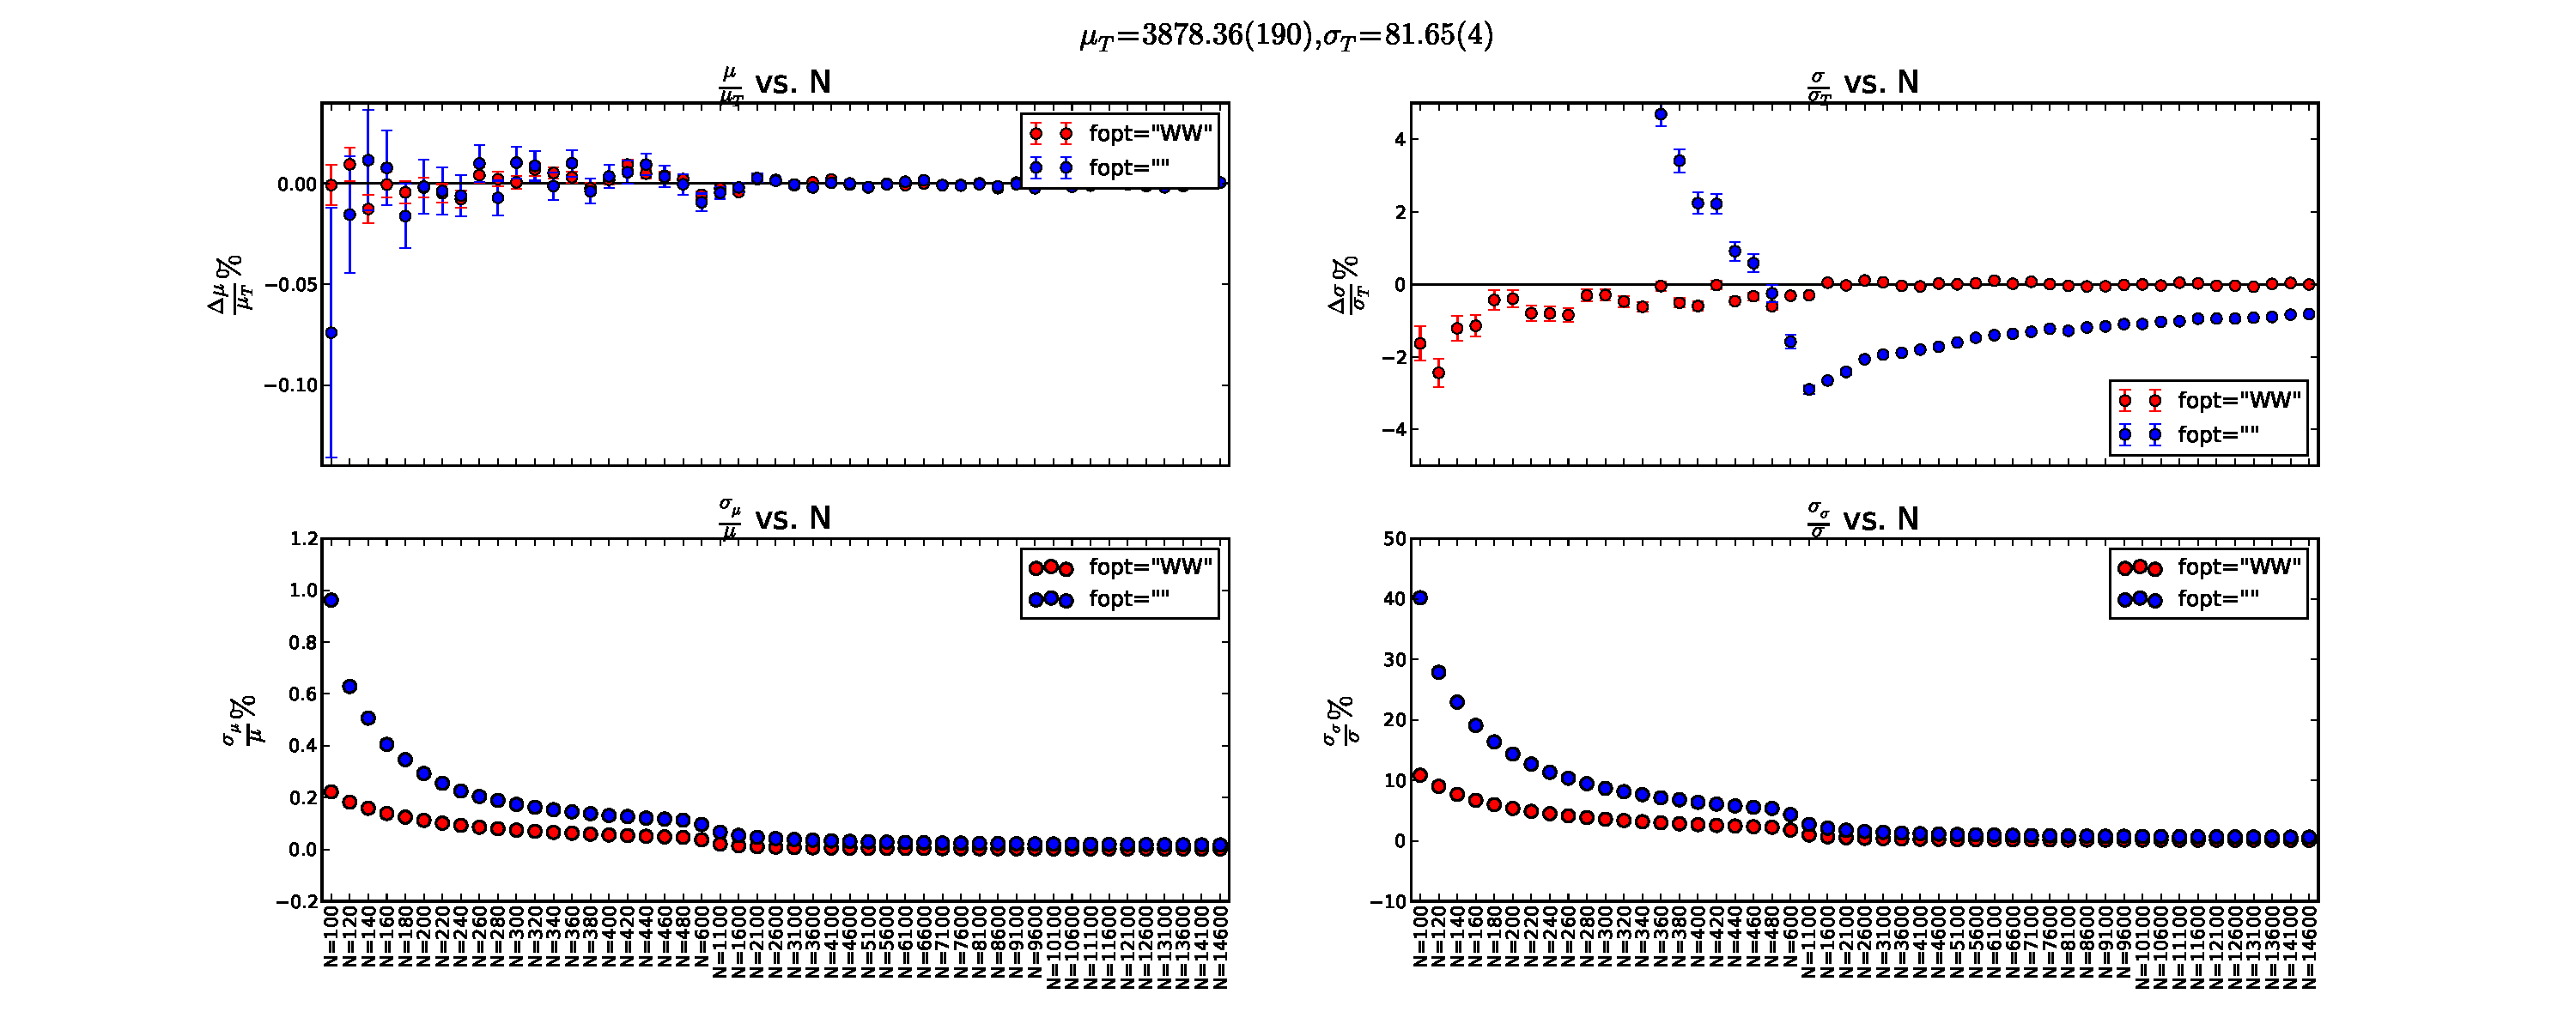
\includegraphics[height=2.5in,width=5.5in]{fit-comp_MU-190_SG-4_fit-opt-WW_binw-025.pdf}
	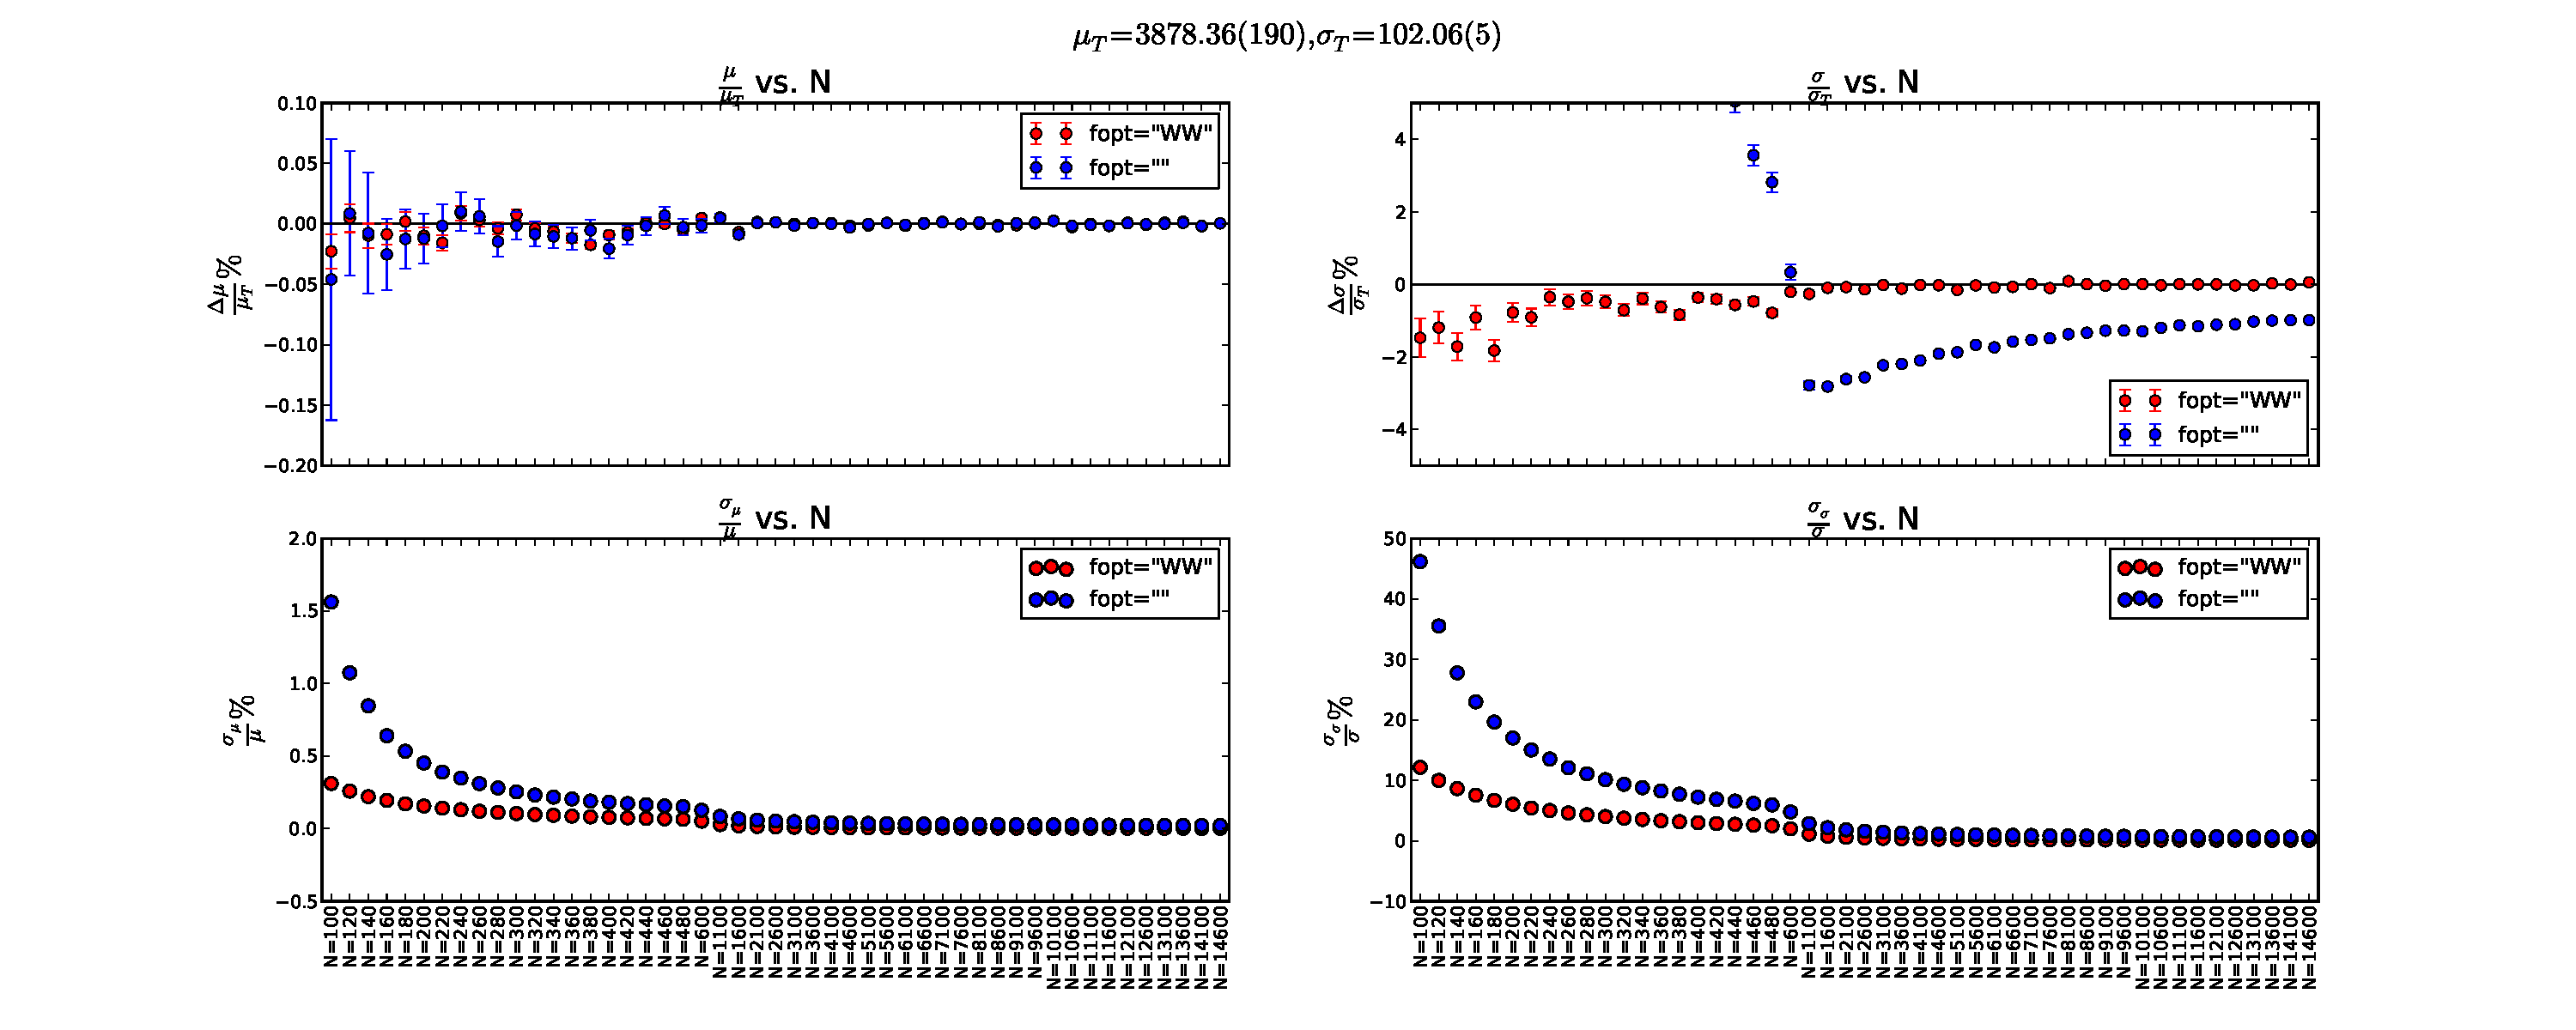
\includegraphics[height=2.5in,width=5.5in]{fit-comp_MU-190_SG-5_fit-opt-WW_binw-025.pdf}
	\caption{Extracted parameters (CSQWW and CSQ)as a function of N and $\sigma_{T}$}
	\label{fig3}
\end{figure*}

\clearpage

\subsection{Effect of error on estimated Time Walk parameters on the time resolution is not determined}
For each 2-day measurement the Time Walk (TW) parameters are estimated (\textit{ref. to sec. in pub.}) and are used to correct each of the TDC measurements for TW (\textit{ref. to formula in pub.}) that go into calculating T (\textit{ref. to formula in pub.}). The error in the estimated TW parameters -- which apart from being statistical can also include non-statistical effects that can vary between measurements --, however, is not accounted for by the width of this T distribution. The only way to estimate the effect of the error of the estimated TW paramaters is to make several 2-day measurements and study the distribution of the respective time resolution measurements. This procedure will be described in detail in the relevant section.

\end{document}